\scanpage{76}
Posant
\[
DR^{pq}=DR^{pq}(X_*)=\operatorname{Ker}(C^{p,q+1}\xrightarrow{\bar T_\bullet}C^{p,q+2}),
\qquad DR^{**}=(DR^{pq})_{p,q\in\unsure{\mathbb Z|\mathbb Z^2}},
\]
on aura donc
\diagram{\begin{tikzcd}[column sep=large]
C^{p,q}\arrow[r,"\bar T_\bullet=u","\text{épi si }p\ne0"']&
DR^{pq}\arrow[d,phantom,"\cap" description]\\
&C^{p,q+1}
\end{tikzcd}}
d'où
\diagram{\begin{tikzcd}
C^{**}\arrow[r,dash,"u"]&DR^{**}\arrow[d,phantom,"\cap\,i" description]&\deleted{\unsure{u}}\\
&C^{**}&
\end{tikzcd}}
\margin{\figure{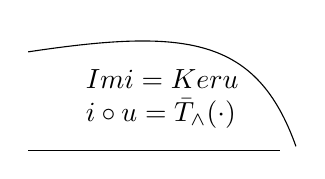
\begin{tikzpicture}
\node[align=left] at (0,0) {$\operatorname{Im}i=\operatorname{Ker}u$\\$i\circ u=\bar T_\wedge(\cdot)$};
\draw (-1.7,.6) .. controls (.3,.9) and (1.2,.8) .. (1.7,-.6);
\draw (-1.7,-.65)--(1.5,-.65);
\end{tikzpicture}}
$(C)\quad i(x)\cdot i(y)=0$}
\margin{(il est évident que $i(DR)\uline{i(uDR)=0}$ donc
$i(DR^{p,q})i(DR^{p',q'})=0$ si \unsure{$p$ ou $p'$}$\ne0$)}
\inserted{et} on aura sur $DR^{**}$ une structure bigraduée différentielle à p.d.
\deleted{telle que}
\inserted{\unsure{comm. gr.}, aux axiomes usuels (\unsure{alternée etc})}
\[
u:C^{**}\longrightarrow\unsure{D^{**}|DR^{**}}
\]
soit compatible avec ces structures
\inserted{et $\left\{\begin{aligned}i(xu(y))&=i(x)y\\i(u(y)x)&=yi(x)\end{aligned}\right.$}.
Ces structures sur $DR^{**}$ sont presque déterminées par ces propriétés, plus celle que l'inclusion
$DR^{**}\subset C^{**}$ est de bidegré $0,1$ et \inserted{anti}commutant à la différentielle -- à la détermination près des produits $xy$ \deleted{$\unsure{x^n}$} et des puissances divisées
$x^{(i)}$ $(i\geq2)$ quand $x,y$ \deleted{\unsure{sont}} de \unsure{degré complémentaire 0},
\margin{\unsure{donc (C) si que|donc (C) i.e.}
\figure{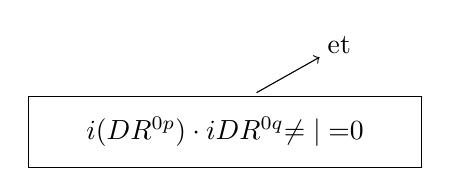
\begin{tikzpicture}
\node at (0,0) {$i(DR^{0p})\cdot iDR^{0q}\unsure{\ne|=}0$};
\draw (-2.5,-.45)--(2.5,-.45)--(2.5,.45)--(-2.5,.45)--cycle;
\draw[->] (.4,.5)--(1.2,.95);
\node at (1.45,1.1) {et};
\end{tikzpicture}}}

(auquel cas on ne peut pas néc. les écrire sous la forme $u(x')$
\inserted{\deleted{\unsure{et}} ou $u(y')$} ($x'$ dans $C^{**}$)).

(\uline{NB} Il est visible que sur \deleted{\unsure{DR}} \unsure{$DR\times DR$}, pour définir
\inserted{\uline{de faç. unique}} une multiplication
\deleted{\unsure{satisfaisant}}
\inserted{\unsure{coïncidant sur} $(\operatorname{Im}u)\times DR$ et $DR\times\operatorname{Im}u$}
\[
u(x,y)=u(x)u(y),\qquad i(xu(y))=i(x)y,\qquad i(u(y)x)=yi(x)
\]
(\deleted{\unsure{car}} la première relation équivaut, en appliquant $i$, à
$\bar T_\bullet(xy)=i(ux\cdot uy)$, d'où en appliquant la deuxième
\[
\bar T\cdot(xy)=(\bar T\cdot x)y
\]
donc il suffit de vérifier l'existence et l'unicité de
$\operatorname{Im}u\times DR-DR$ et $DR\times\operatorname{Im}u-DR$
satisfaisant les rel. 2 et 3. Or pour la $2^{\text{ème}}$, il suffit de montrer que

a) $i(x)y\inserted{=xy}\in\deleted{\operatorname{Ker}\unsure{\bar T}}DR=\operatorname{Ker}(\bar T_\wedge)$

car $\bar T(xy)=(\bar T x)y=0$ car $\bar T x=0$ puisque $x\in DR$

b) $i(x)y\inserted{=xy}$ ne dépend que de $x\in DR$ et de $uy\in\unsure{BR|DR}$,

car si $uy)=0$ i.e. $\bar T y=0$, i.e. $y\in DR$, on a
$xy=0$ -- Idem pour 3.
\margin{75}
